\documentclass[a4paper,10pt]{article}
\usepackage[utf8]{inputenc}
\usepackage{markdown}

%opening
\title{Offensive security\\lab-report}
\author{Moritz Rupp}

\begin{document}

\maketitle

\begin{abstract}
\noindent This document contains reports about the laboratory of the 5th semester module offensive security. 
\end{abstract}
\tableofcontents

\newpage
\section{Lab2}
\subsection{Exercise 2.2}
\begin{center}
\textbf{https://www.hs-albsig.de} 
\end{center}
\$\raisebox{-0.9ex}{\~{}} nslookup hs-albsig.de \\
IP: 94.186.153.201\\ 


\noindent\$\raisebox{-0.9ex}{\~{}} nmap -sC -sV -oA 94.186.153.201\\
Open ports: 80(HTTP), 443(HTTPS)\\
Server: nginx 1.16.1\\
HTTP Version: 1.1 
\\
\\
\$\raisebox{-0.9ex}{\~{}} whois hs-albsig\\
SOA: ns.hs-albsig.de. (141.87.109.5)\\  
Namerserver:
\begin{itemize}
\item Nserver: dns1.belwue.de
\item Nserver: dns3.belwue.de
\item Nserver: dns5.belwue.de
\item Nserver: ns.hs-albsig.de 141.87.109.5
\end{itemize}
 
\noindent\$\raisebox{-0.9ex}{\~{}} fierce   --domain hs-albsig --wide\\
Some of the found subdomains, all belonging to the main host of hs-albsig!\\
To see the full list, take a look at the file 'fierceoutput.txt'.  
\\
\begin{itemize}
 \item helpdesk.hs-albsig.de. - 141.87.114.175
 \item info.hs-albsig.de. - 141.87.114.205
 \item konferenz.hs-albsig.de. - 141.87.115.200
 \item intern.hs-albsig.de. - 141.87.109.198
 \item autodiscover.hs-albsig.de. - 141.87.109.198
 \item h1crelay1.hs-albsig.de. -141.87.109.200
 \item intranet.hs-albsig.de. - 141.87.109.198
 \item jobs.hs-albsig.de. - 62.204.161.138
 \item live.hs-albsig.de. - 141.87.190.3
 \item login.hs-albsig.de. - 194.98.248.75
 \item mail.hs-albsig.de. - 141.87.114.190
 \item mailig.hs-albsig.de. - 54.73.30.56
 \item ntp.hs-albsig.de. - 141.87.190.5
 \item pki.hs-albsig.de. - 141.87.109.3
 \item proxy.hs-albsig.de. - 141.87.109.4
 \item datascience.hs-albsig.de. - 141.87.109.223
  

\end{itemize}

\vspace{10mm}
\noindent The same results can be achived via recon-ng and the hackertarget module.\\
\newline
\noindent\$\raisebox{-0.9ex}{\~{}} recon-ng\\
\$\raisebox{-0.9ex}{\~{}} marketplace search hackertarget\\
\$\raisebox{-0.9ex}{\~{}} marketplace install hackertarget\\
\$\raisebox{-0.9ex}{\~{}} modules load hackertarget\\ 
\$\raisebox{-0.9ex}{\~{}} options set SOURCE hs-albsig.de\\
\$\raisebox{-0.9ex}{\~{}} run

\vspace{5mm}
\noindent \textbf{More interesting information about the host hs-albsig.de:\\
Common http security headers are missing!}\\
\begin{itemize}
\item Content-security-policy(csp)
\item HTTP Strict Transport Security (HSTS)
\item Cross Site Scripting Protection (X-XSS)
\item X-Frame-Options
\item X-Content-Type-Options(no sniff)
 \end{itemize}


\newpage
\subsection{Exercise 2.3}
Out of my 10 email adresses, 3 have been part of a leagage.
A paid licence is required to view the actuall document content tho.
But it is possible to see the origin of the leagage.\\
Leagage origins:
\begin{itemize}
 \item Dailymotion.com
 \item Dropbox.comment
 \item Linux-Foren.com
 \item RepZ.eu
 \item hqcombo.top
\end{itemize}
\vspace{3mm}
Phonebook.cz was able to find over 500 email adresses of albstadt uni members. The majority of leagages matched the above listing.
With the help of tools and websites such as lullar.com, mSpy and peekyou i was able to find the according social media accounts of several email adresses. 

\subsection{Exercise 2.4}
Searching for company related documents with metagoofil:\\
\noindent\$\raisebox{-0.9ex}{\~{}} metagoofil -t pdf -d hs-albsig\\

\noindent Metagoofil found several hundred uni related documents including sensitive files like exams and salary information.\\
Exemplary scan of one of the found documents with \textbf{exiftool}. 
\begin{center}

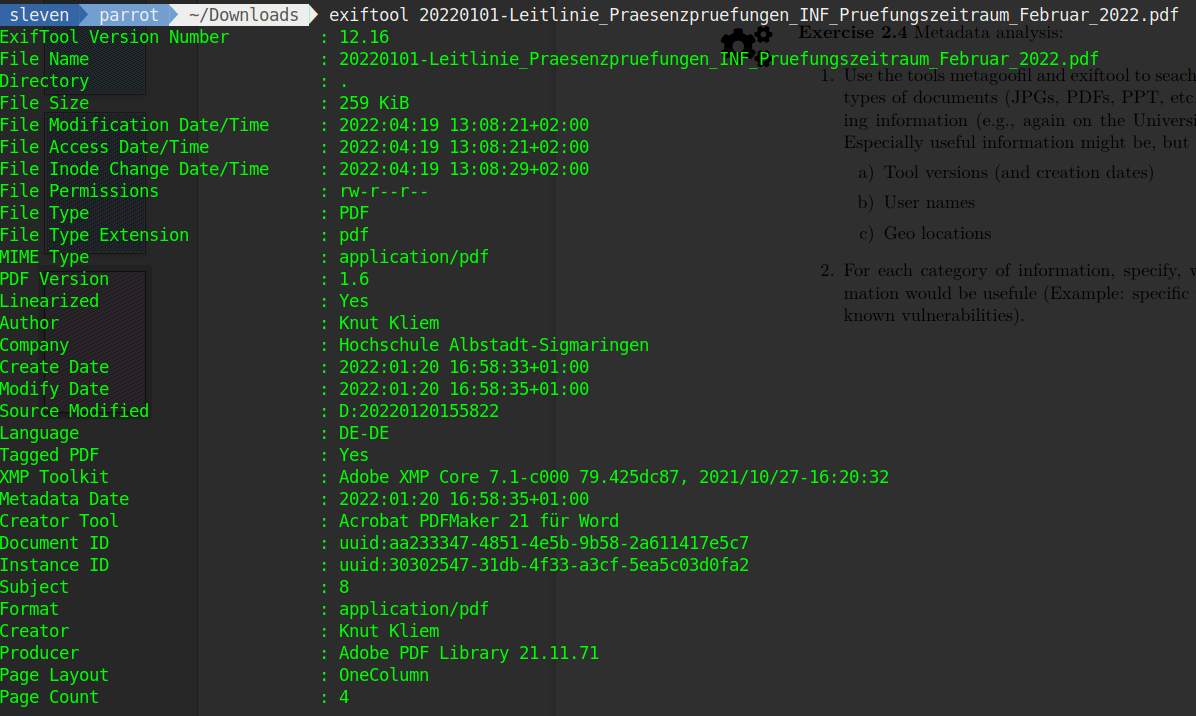
\includegraphics[scale=0.35]{exif.png} 
\end{center}
\textbf{Particular interesting information:}\\
File Size: If much bigger than expected, that could be a sign for more hidden meta data like steganography etc.\\
File modification/access date/time: Was the file created prior to certain vulnabilities/patches etc.?! \\
MIME Type: Is the file the format it claims to be?! Executable malware can be hidden as a fake format like pdf or jpg.\\
Creator: Can be used to ascertain to what department someone belongs to. This can further be used for more osint.\\
Geotag: If pictures show sensitive infrastrucure of a company(server, admin rooms etc.) the geotag can be used to find the real location. This can be used for stuff like dumbster diving etc.  \\
\vspace{3mm}

\noindent It can be noticed that most documents didnt include sensitive information such as geotags etc.
\end{document}
